\newcommand{\package}{\emph}

\setcounter{chapter}{1}
\setcounter{section}{0}

\section{a-b}


\begin{figure}[h!]
  \centering 
  \subfloat[$t=500$, initial
  cond.~$X_{01}$]{\label{fig:plot_1A}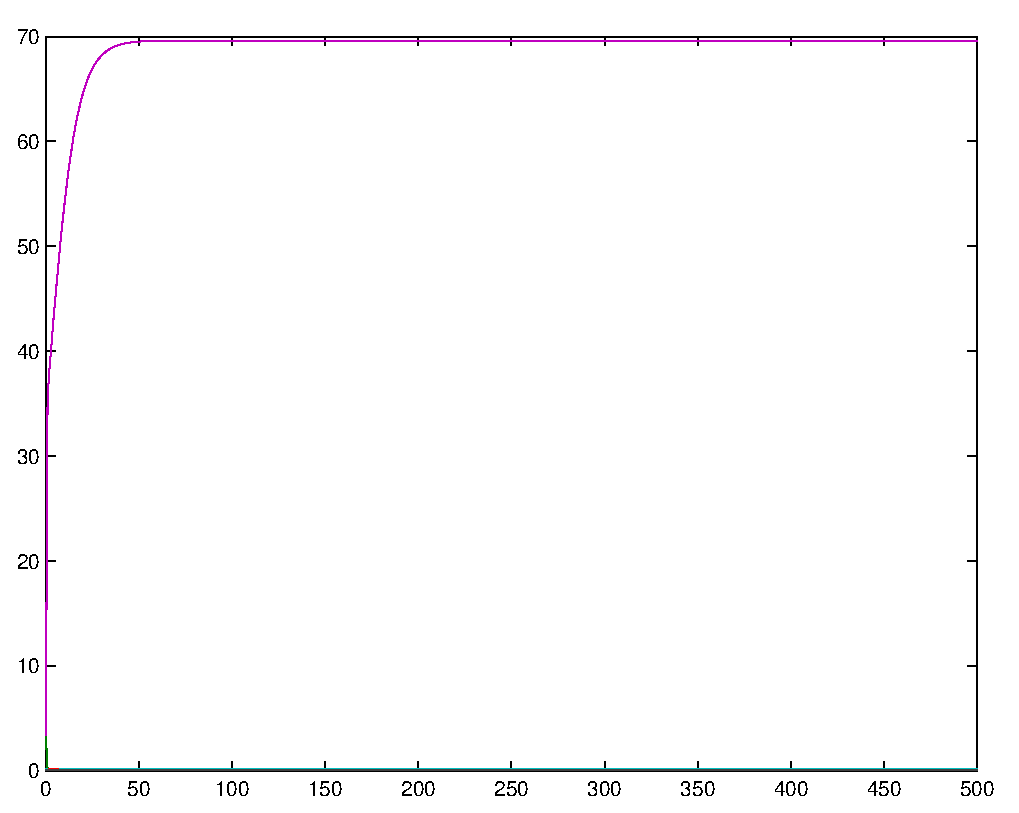
\includegraphics[scale=0.43]{plot_1A}} ~ 
  \subfloat[$t=500$, initial
  cond.~$X_{02}$]{\label{fig:plot_1B}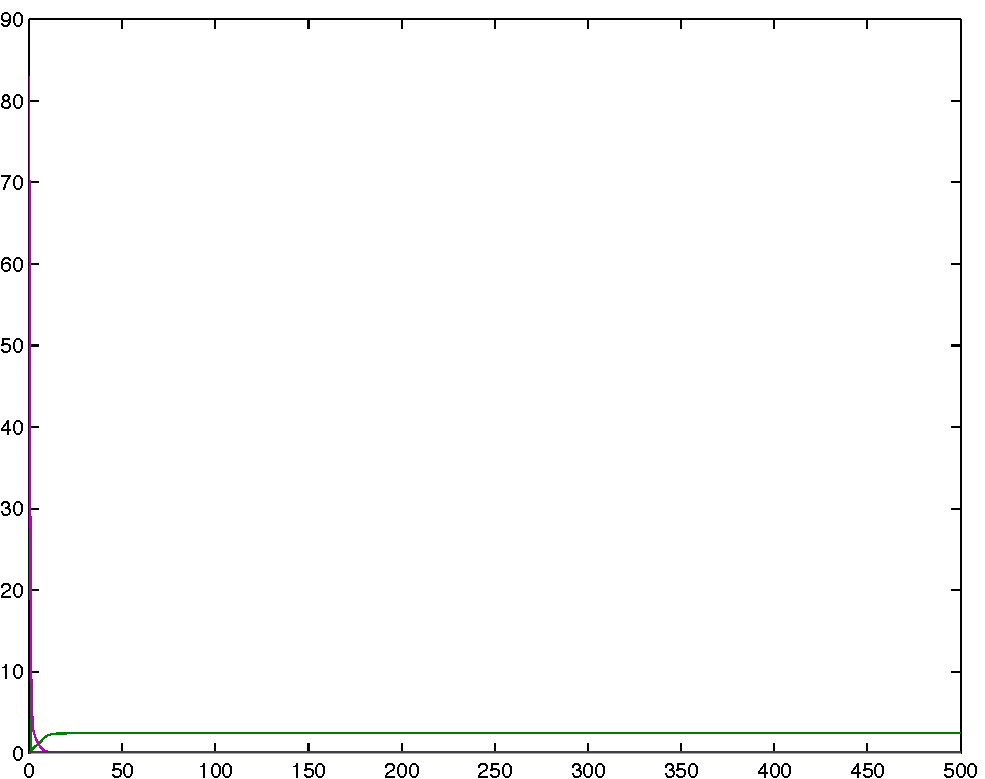
\includegraphics[scale=0.43]{plot_1B}} \\
  \subfloat[]{\begin{tabular}{l|cc}
					& C/(nM) & No. \\
					\hline
					$P_1$ & $0.0392$ &  $0$ \\    
					$P_2$ & $69.6284$ & $419$ \\
					\end{tabular}} ~~~~~~~~~~~~~~~~~~~~~~~~~~~~~~
  \subfloat[]{\begin{tabular}{l|cc}
					& C/(nM) & No. \\
					\hline
					$P_1$ & $2.4285$ &  $14$ \\    
					$P_2$ & $0.1400$ & $0$ \\
					\end{tabular}}
  \caption{Concentration evolution plots (espressed in nM) for different
  initial conditions ($X_{01}$ and $X_{02}$) until $t=500$. Values of protein
  $P_1$ and $P_2$ levels at steady state.}
  \label{fig:plot_tab_det_c01}
\end{figure}

Bistability is well detected in plot \ref{fig:plot_1B} for this set of
parameters.

\setcounter{chapter}{2}
\setcounter{section}{0}
\section{a}
Set of values for the stochastic rate constants ($\hat{k}$).

\begin{equation}
set\_SRC = [k_1~k_{c1}^+~k_{c1}^-~k2~k_{c2}^+~k_{c2}^-~k_{c3}^+~k_{c3}^-~d1~d2]  
\end{equation}
\begin{equation}
set\_SRC = [100~0.1661~1~1000~0.1661~1~16.6113~1~6~2];
\end{equation}

\section{b}
Computed values of the \emph{propensities} associated to each reaction channel
at $t=0$ for initial conditions $X_{01}$, $X_{02}$, $X_{03}$, $X_{04}$.

\begin{table}[h!]
\begin{center}
\begin{tabular}{|l|rrrr|}
\hline
& $X_{01}$ & $X_{02}$ & $X_{03}$ & $X_{04}$ \\
\hline
R1 & 0.0100 & 0.0100 & 0.1000 & 0.1000 \\
R2 & 0.0003 &0.0083 & 0.0033 & 0.0830 \\
R3 & 0.0000 & 0.0000 & 0.0000 & 0.0000 \\
R4 & 0.1000  & 0.1000 & 1.0000 & 1.0000 \\
R5 & 0.0003 & 0.0083 & 0.0033 & 0.0830 \\
R6 & 0.0000 & 0.0000 & 0.0000 & 0.0000 \\
R7 & 0.0000 & 0.0000 & 0.0000 & 0.0000 \\
R8 & 0.0000 & 0.0000 & 0.0000 & 0.0000 \\
R9 & 0.0120 & 0.3000 & 0.0120 & 0.3000 \\
R10 & 0.0040 & 0.1000 & 0.0040 & 0.1000 \\
\hline
\bottomrule
\end{tabular}
\caption{Propensities (all the values have to be multiplied for
$1.0E+04$)}
\end{center}
\end{table}					

\section{c}

\begin{table}[h!]
\begin{center}
\begin{tabular}{|l|rrrrrrr|}
\hline
R1 & 0 & 1 & 0 & 0 & 0 & 0 & 0 \\
\hline
R2 & $-1$ & 0 & 1 & 0 & $-1$ & 0 & 0 \\
\hline
R3 & 1 &0 &$-1$ &0 &1 &0 &0\\
\hline
R4 & 0 &0 &0 &0 &1 &0 &0\\
\hline
R5 & 0 &$-1$ &0 &$-1$ &0 &1 &0\\
\hline
R6 & 0 &1 &0 &1 &0 &$-1$ &0\\
\hline
R7 & 0 &$-1$ &0 &0 &0 &$-1$ &1\\
\hline
R8 & 0 &1 &0 &0 &0 &1 &$-1$\\
\hline
R9 & 0 & $-1$ &0 &0 &0 &0 &0\\
\hline
R10 & 0 &0 &0 &0 &$-1$ &0 &0\\
\hline
\bottomrule
\end{tabular}
\caption{State change vectors for each reaction channel}
\end{center}
\end{table}					
\newpage
\section{d}

\begin{figure}[h!]
 \centering
    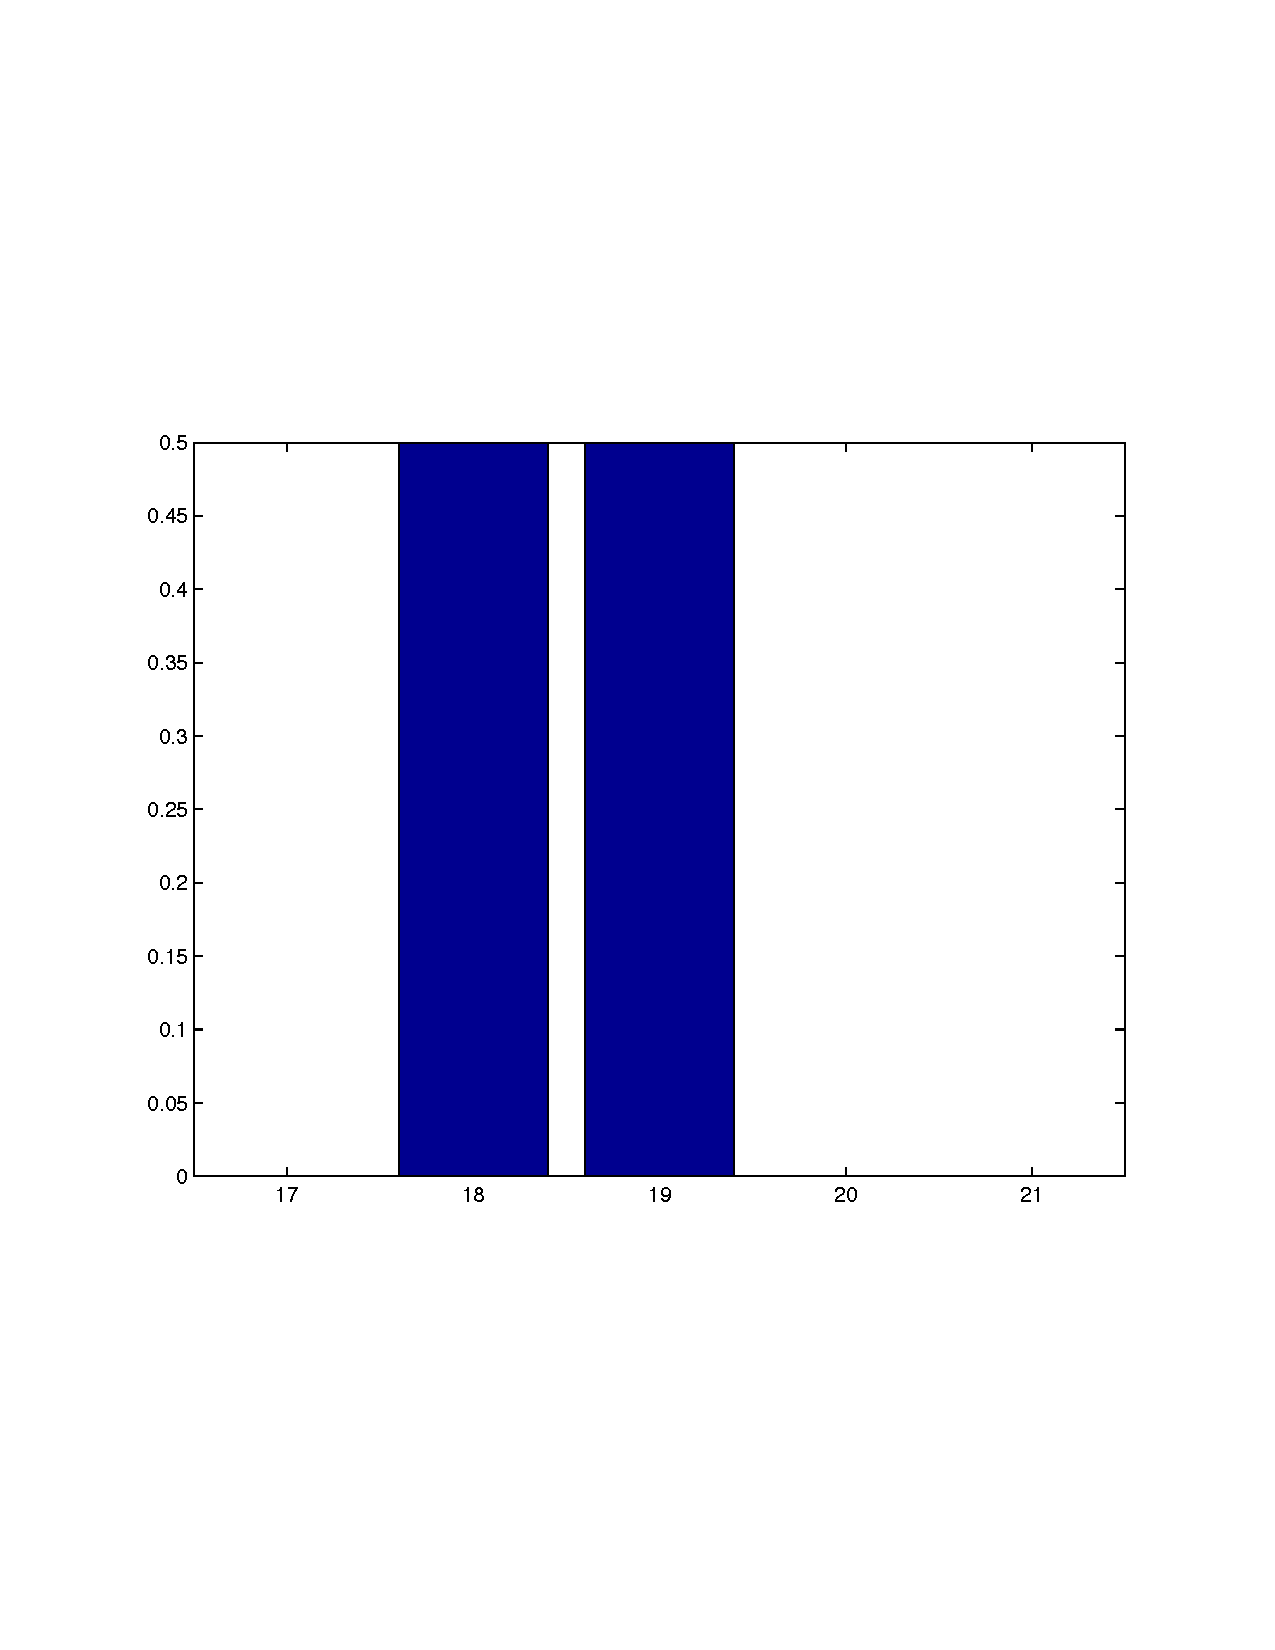
\includegraphics[scale=0.5]{plot_2E} \caption{Histogram illustrating the
    probability distribution for the number of molecules of protein $P_1$ after
    reaching the steady state.}
	\label{fig:plot_2E}
\end{figure}
\newpage
\setcounter{chapter}{3}
\setcounter{section}{0}
\section{Optional}
\begin{figure}[h!]
  \centering \subfloat[Deterministic simulation for initial conditions
  $X_{03}$]{\label{fig:plot_DC3}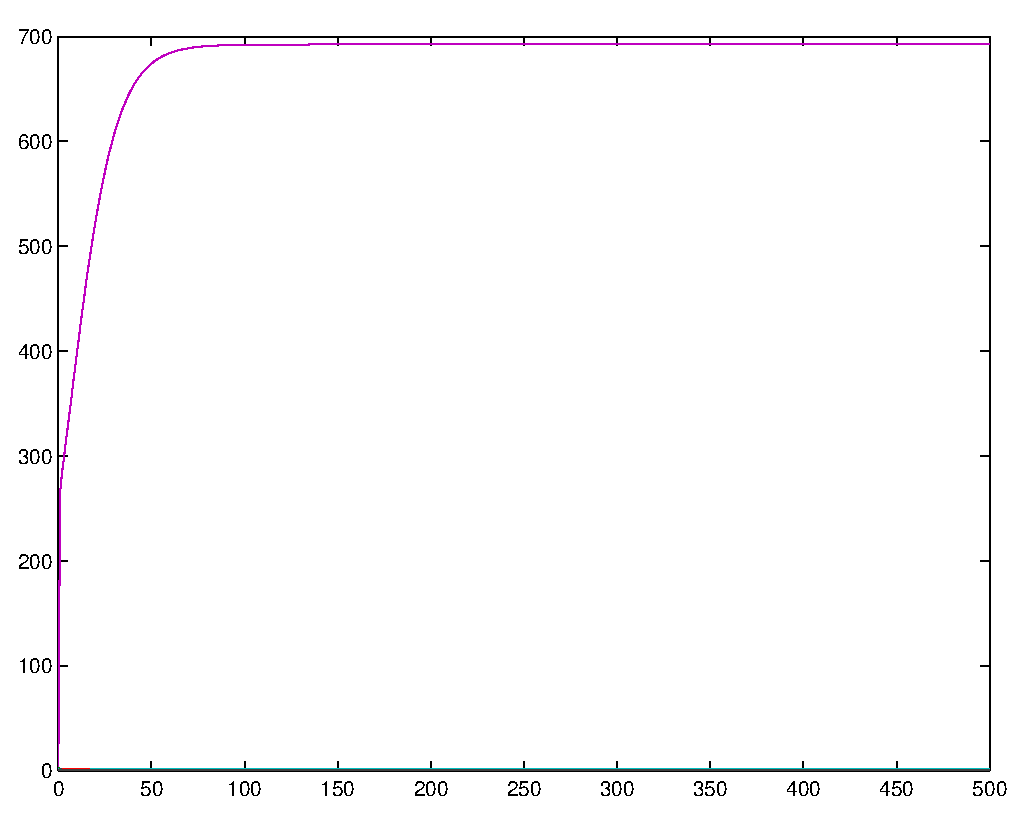
\includegraphics[scale=0.44]{plot_3_D_C3}} ~
  \subfloat[Deterministic simulation for initial conditions
  $X_{04}$]{\label{fig:plot_DC4}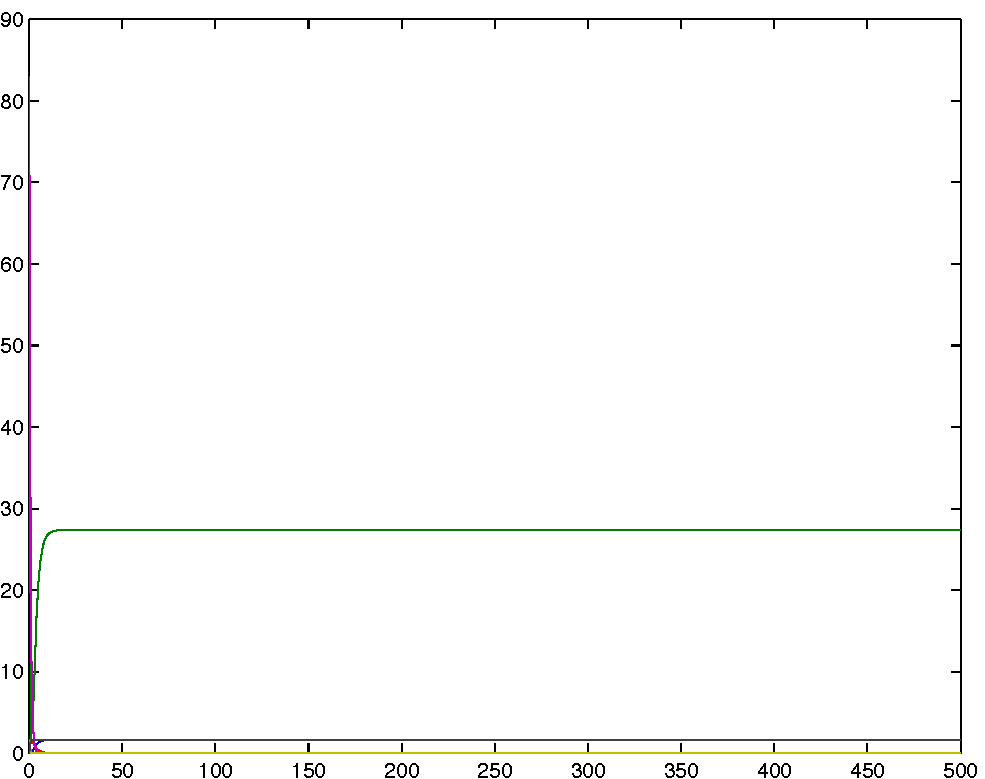
\includegraphics[scale=0.44]{plot_3_D_C4}}
  
  \subfloat[]{\begin{tabular}{l|cc}
					& C/(nM) & No. \\
\hline
					$P_1$ & $0.0399$ &  $0$ \\    
					$P_2$ & $692.5645$ & $4169$ \\
\end{tabular}} ~~~~~~~~~~~~~~~~~~~~~~~~~~~~~~
  \subfloat[]{\begin{tabular}{l|cc}
					& C/(nM) & No. \\
\hline
					$P_1$ & $27.3823$ &  $164$ \\    
					$P_2$ & $0.0111$ & $0$ \\
					\end{tabular}} \\
  \caption{Concentration evolution plots (espressed in nM) for different initial
  conditions ($X_{03}$ and $X_{04}$) until $t=500$. Values of protein $P_1$ and
  $P_2$ levels at steady state.}
  \label{fig:plot_detstosim_c03c04}
\end{figure}

\begin{figure}[h!]
 \centering
    \label{fig:plot_SC3}
    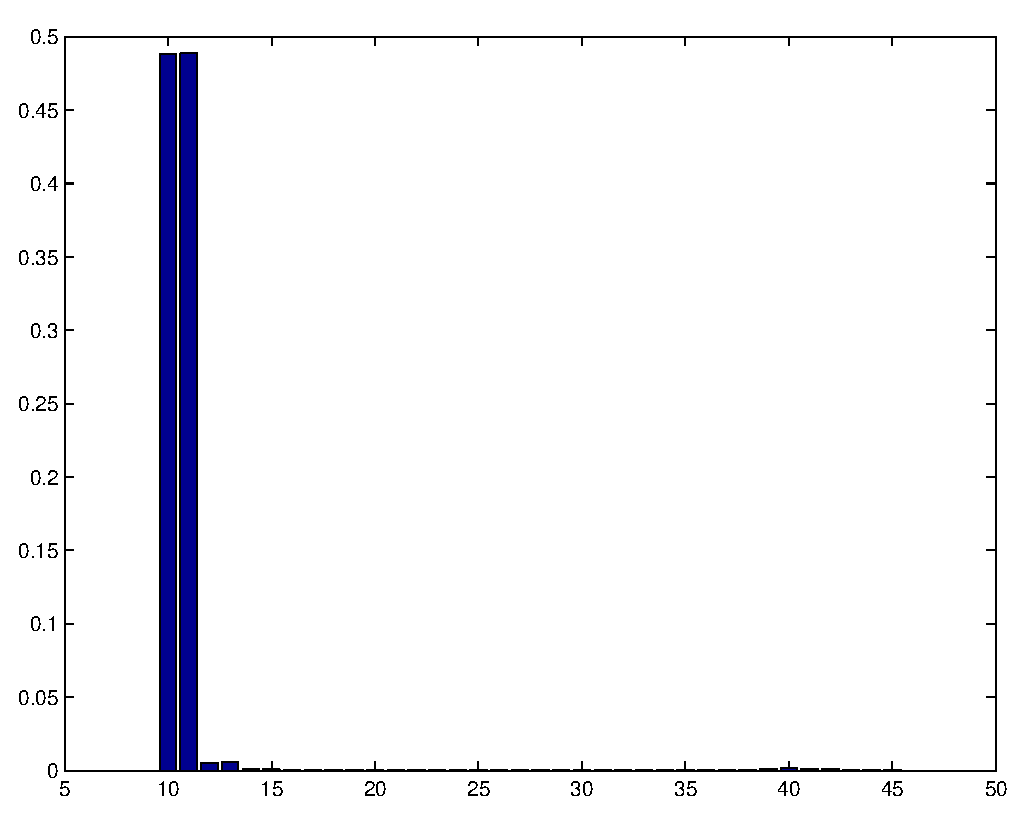
\includegraphics[scale=0.44]{plot_3_S_C03}
    \caption{Histogram illustrating the
    probability distribution for the number of molecules of protein $P_1$ after
    reaching the steady state for initial condition $P_{03}$}
	
\end{figure}